
%================================
\subsection{Resultados de las pruebas del algoritmo optimizado por compilador}
\label{sec:Resultados_compilador}

Para este algoritmo se usaron las siguientes opciones de compilación: -O3, -funroll-loops, -fomit-frame-pointer y -march=native. Estas opciones permiten al compilador realizar optimizaciones agresivas, como la eliminación de código innecesario, el desenrollado de bucles y la generación de código específico para la arquitectura del procesador. Estas optimizaciones pueden mejorar significativamente el rendimiento del algoritmo, especialmente en casos donde se realizan muchas iteraciones o se manejan grandes cantidades de datos. 

El signigicado de cada bandera es el siguiente:
\begin{itemize}
   \item \textbf{-O3:} Esta bandera habilita un nivel de optimización agresivo, permitiendo al compilador aplicar una amplia gama de técnicas para mejorar el rendimiento del código.
   \item \textbf{-Wall:} Activa la mayoría de las advertencias del compilador, lo que ayuda a identificar posibles problemas en el código que podrían afectar su rendimiento o funcionalidad.
   \item \textbf{-march=native:} Permite al compilador generar código optimizado para la arquitectura específica del procesador en el que se está compilando, aprovechando las características y capacidades de hardware disponibles.
   \item \textbf{-funroll-loops:} Habilita el desenrollado de bucles, lo que puede mejorar el rendimiento al reducir la sobrecarga de control de bucle y aumentar la paralelización de las instrucciones.
   \item \textbf{-flto:} Habilita la optimización a nivel de enlace, lo que permite al compilador realizar optimizaciones globales en todo el programa, incluso entre diferentes archivos de código fuente.
   \item \textbf{-ffast-math:} Permite al compilador realizar optimizaciones agresivas en operaciones matemáticas, lo que puede mejorar el rendimiento a costa de la precisión en algunos casos como la evaluación de funciones trigonométricas.
   \item \textbf{-fomit-frame-pointer:} Indica al compilador que no utilice un puntero de marco para las funciones, es decir, que no cree un marco de pila para cada función, lo que puede mejorar el rendimiento al reducir la cantidad de instrucciones necesarias para gestionar la pila de llamadas.
\end{itemize}


Se realizaron las pruebas para el algoritmo secuencia optimizado por compilador y estos fueron los resultados obtenidos:

\begin{table}
   \centering
   
\includegraphics[width=1\textwidth]{images/tables/compiler_time.png}
   \caption{Resultados del algoritmo secuencial optimizado por compilador}
   \label{tab:compiler}
\end{table}

\begin{table}[H]
   \centering
   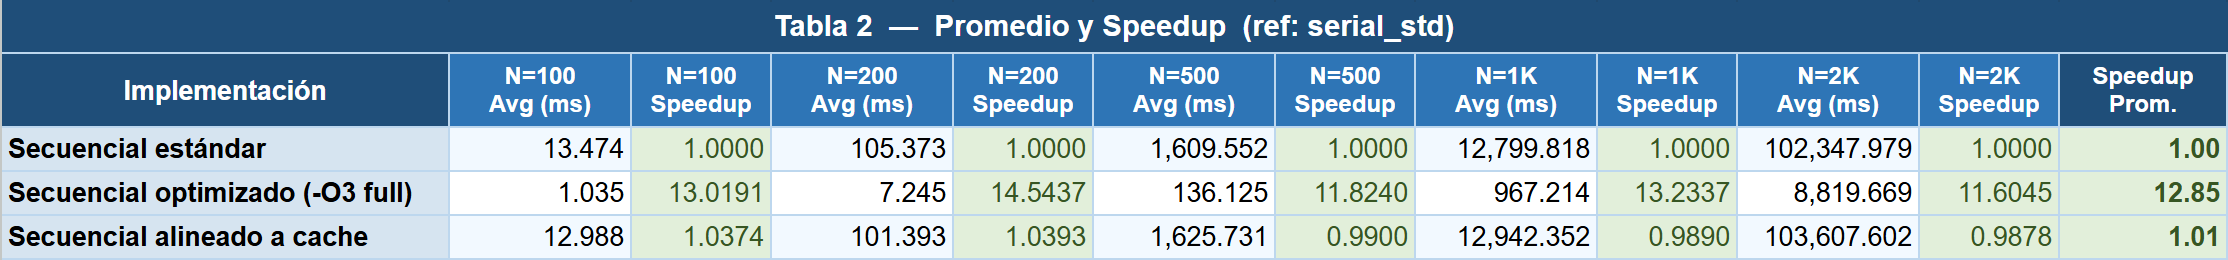
\includegraphics[width=1\textwidth]{images/tables/serial_speedup.png}
   \caption{Speedup del algoritmo secuencial optimizado por compilador}
   \label{tab:compiler_speedup}
\end{table}


\begin{table}[H]
   \centering
   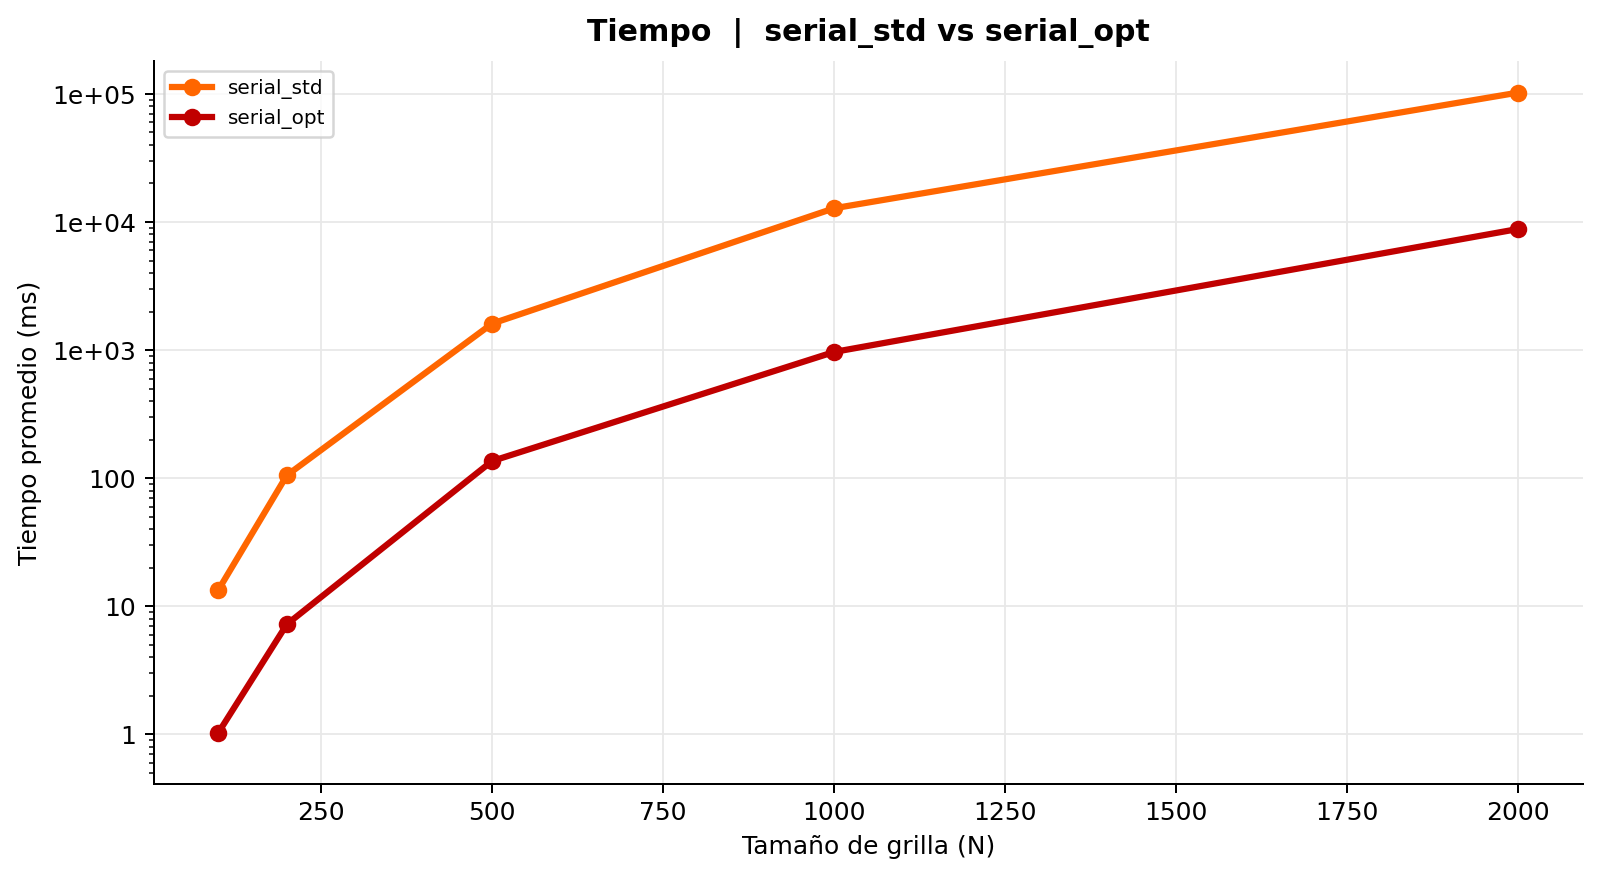
\includegraphics[width=1\textwidth]{images/charts/compiler_time.png}
   \caption{Comparación del tiempo de ejecución entre el algoritmo secuencial y el algoritmo secuencial optimizado por compilador}
   \label{tab:compiler_time}
\end{table}

\begin{figure}[H]
   \centering
   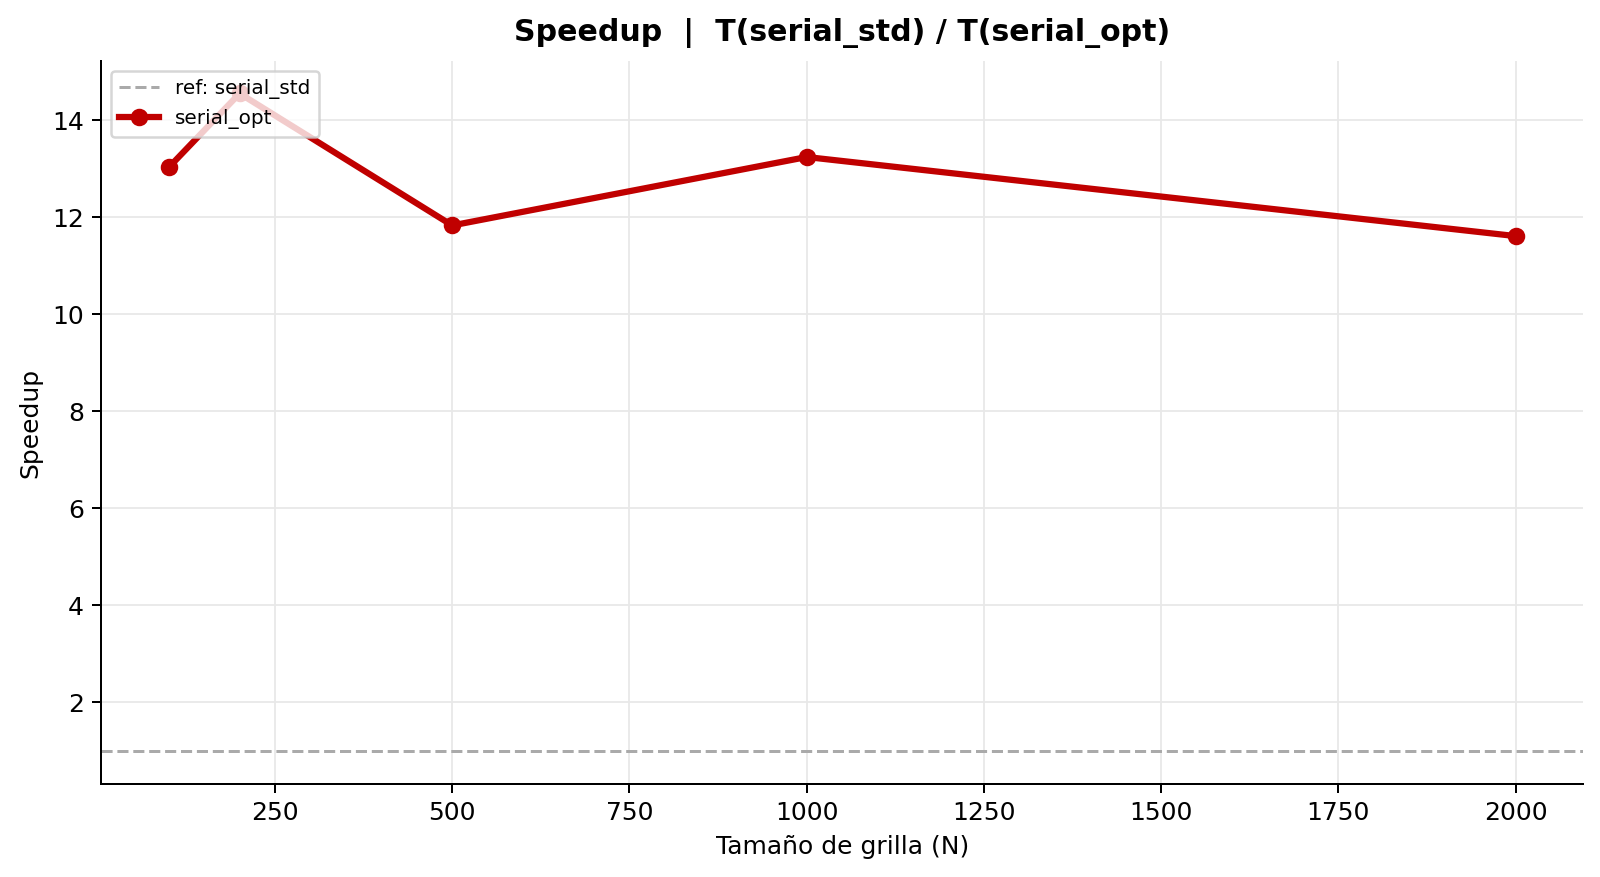
\includegraphics[width=1\textwidth]{images/charts/compiler_sp.png}
   \caption{Comparación del speedup entre el algoritmo secuencial y el algoritmo secuencial optimizado por compilador}
   \label{fig:chart_compiler_speedup}
\end{figure}